\section{The Born--Oppenheimer approximation}\label{sec:5.1}

The optical phonon of silicon at the zone center vibrates at \SI{15.5}{THz}~\cite{nilsson1972study}, an energy of \SI{64.1}{meV} and a period of \SI{64.5}{fs}. An electron excited across the gap of \SI{1.17}{eV} evolves on the time $2\pi/\Eg = \SI{3.5}{fs}$, eighteen times faster. During one swing of the nuclei the electrons have time to settle, many times over, into the lowest state compatible with where the nuclei happen to be. The crystal then behaves as the static lattice of \cref{sec:3.1} with the nuclei now allowed to move, slowly. This separation of the slow nuclei from the fast electrons is due to Born and Oppenheimer~\cite{born1927quantentheorie}, in the form that Born and Huang gave it for crystals~\cite[App.~VIII]{born1954dynamical}; the derivations of this section are written out in \cref{app:D.13}.

\subsection{Adiabatic states}

We start from the Coulomb Hamiltonian of electrons and point nuclei, \cref{eq:2.3-HC}. In a crystal it is natural to label the nucleus $I$ of \cref{sec:2.3} by its cell and its place in the cell. In the cell at the Bravais vector $\vect{R}$, the nucleus of species $\kappa$ sits at
\begin{equation}
  \vect{X}_I = \vect{R} + \vect{\tau}_\kappa + \vect{u}_{\vect{R}\kappa} ,
  \label{eq:5.1-X}
\end{equation}
where $\vect{\tau}_\kappa$ is its basis position in the cell (\cref{sec:3.1}) and $\vect{u}_{\vect{R}\kappa}$ its displacement. We write $u$ for the set of all displacements and $\nabla_{\vect{R}\kappa} = \partial/\partial\vect{u}_{\vect{R}\kappa}$. The equilibrium positions, about which $u$ is measured, are fixed below. Of the terms of \cref{eq:2.3-HC}, only the kinetic energy of the nuclei contains $\nabla_{\vect{R}\kappa}$. We separate it from the rest,
\begin{equation}
  H = -\sum_{\vect{R}\kappa}\frac{\nabla_{\vect{R}\kappa}^2}{2M_\kappa} + H_{\mathrm{el}}(u), \qquad
  H_{\mathrm{el}}(u) = T_e + V_{ee} + V_{eN}(u) + V_{NN}(u) ,
  \label{eq:5.1-H}
\end{equation}
with $T_e$ the kinetic energy of the electrons, the first term of \cref{eq:2.3-HC}, and $V_{ee}$, $V_{eN}$ and $V_{NN}$ the electron--electron, electron--nucleus and nucleus--nucleus terms of the bracket of \cref{eq:2.3-HC}. At fixed $u$, $H_{\mathrm{el}}(u)$ acts on the electron coordinates alone, which we collect in $r$, and the displacements $u$ enter $H_{\mathrm{el}}(u)$ as a set of parameters. The eigenstates of $H_{\mathrm{el}}(u)$ are the \emph{adiabatic states},
\begin{equation}
  H_{\mathrm{el}}(u)\,\Psi_i(r;u) = E_i(u)\,\Psi_i(r;u) ,
  \label{eq:5.1-adiabatic}
\end{equation}
orthonormal at every $u$. Each is a state of all the electrons with the nuclei held at the positions $u$. In the absence of a magnetic field $H_{\mathrm{el}}$ is real and the $\Psi_i$ can be chosen real, which we assume.

The adiabatic states are complete in $r$ at each $u$, and an exact state of electrons and nuclei can be expanded in them with $u$-dependent coefficients,
\begin{equation*}
  \Psi(r,u) = \sum_i\Psi^{\mathrm{nuc}}_i(u)\,\Psi_i(r;u) .
\end{equation*}
The coefficients $\Psi^{\mathrm{nuc}}_i$ are nuclear wavefunctions, one for each electronic state, and so far nothing has been approximated. Inserting the expansion into $H\Psi = E\Psi$ and projecting on $\Psi_j$ at fixed $u$ (\cref{app:D.13}) leads to coupled equations for the nuclear wavefunctions,
\begin{equation}
  \Bigl[-\sum_{\vect{R}\kappa}\frac{\nabla_{\vect{R}\kappa}^2}{2M_\kappa} + E_j(u)\Bigr]\Psi^{\mathrm{nuc}}_j + \sum_i\mathcal{N}_{ji}\,\Psi^{\mathrm{nuc}}_i = E\,\Psi^{\mathrm{nuc}}_j ,
  \label{eq:5.1-coupled}
\end{equation}
in which the electronic states couple to each other only through the operators
\begin{equation}
  \mathcal{N}_{ji} = -\sum_{\vect{R}\kappa}\frac{1}{2M_\kappa}\Bigl[2\,\langle\Psi_j|\nabla_{\vect{R}\kappa}\Psi_i\rangle\cdot\nabla_{\vect{R}\kappa} + \langle\Psi_j|\nabla_{\vect{R}\kappa}^2\Psi_i\rangle\Bigr] .
  \label{eq:5.1-N}
\end{equation}
These are the \emph{nonadiabatic couplings}: the first-derivative (or derivative) coupling, which acts on the nuclear wavefunction through $\nabla_{\vect{R}\kappa}$, and the second-derivative (or scalar) coupling. The brackets are integrals over $r$ and functions of $u$. Both couplings exist because the electronic state changes as the nuclei move, and both carry the factor $1/M_\kappa$.

The \emph{Born--Oppenheimer approximation} drops the nonadiabatic couplings. The electrons then stay in one adiabatic state (for an insulator at low temperature, the ground state), and the nuclei move in its energy:
\begin{equation}
  \Bigl[-\sum_{\vect{R}\kappa}\frac{\nabla_{\vect{R}\kappa}^2}{2M_\kappa} + E^{\mathrm{ad}}(u)\Bigr]\Psi^{\mathrm{nuc}}_0 = E\,\Psi^{\mathrm{nuc}}_0 , \qquad
  E^{\mathrm{ad}}(u) \equiv E_0(u) , \qquad
  \Psi \simeq \Psi^{\mathrm{nuc}}_0(u)\,\Psi_0(r;u) .
  \label{eq:5.1-BO}
\end{equation}
The ground-state energy of the electrons at fixed nuclei, with the repulsion of the nuclei included, has become the potential energy of the nuclei. It is the \emph{potential-energy surface}, or Born--Oppenheimer energy surface, $E^{\mathrm{ad}}(u)$, a function of the $3n_{\mathrm{at}}N$ nuclear coordinates for a crystal of $N$ cells, each with $n_{\mathrm{at}}$ nuclei. The physical picture is a slow nucleus pulling a cloud of electrons that rearranges instantly: the electrons follow the nuclei adiabatically, never get excited, and pass to the nuclei only the energy of their ground state. The rest of this chapter treats phonons, from their frequencies to their anharmonic decay, and every result it obtains is a statement about the shape of $E^{\mathrm{ad}}$ and about quantum mechanics on that surface. Born and Huang keep the diagonal term $\mathcal{N}_{00}$ as a small correction to $E^{\mathrm{ad}}$ and call the result the adiabatic approximation~\cite[App.~VIII]{born1954dynamical}. The field uses ``adiabatic'' and ``Born--Oppenheimer'' interchangeably, and so do we, since $\mathcal{N}_{00}$ is negligible (\cref{app:D.13}). The off-diagonal couplings $\mathcal{N}_{j\ne0,0}$ are what let a moving nucleus excite the electrons; they are the subject of \cref{sec:6.1}.

In a density-functional code, $E^{\mathrm{ad}}$ at a given set of nuclear positions is the Kohn--Sham total energy plus the repulsion of the nuclei (evaluated as an Ewald sum), and every code prints it as its standard output. Evaluating $E^{\mathrm{ad}}$ at displaced positions is the frozen-phonon method, and density-functional perturbation theory (\cref{sec:5.4}) computes the derivatives of $E^{\mathrm{ad}}$ at equilibrium directly. The Born--Oppenheimer approximation enters these calculations at one point only: the electrons are kept in their ground state at every configuration of the nuclei~\cite[Sect.~III\,A]{giustino2017electron}.

\subsection{Equilibrium positions and clamped nuclei}

The nuclei of a crystal at rest sit at a minimum of the energy surface. We choose the equilibrium positions $\vect{R} + \vect{\tau}_\kappa$ so that $u = 0$ is that minimum, $\nabla_{\vect{R}\kappa}E^{\mathrm{ad}} = 0$ for every nucleus. In silicon, each atom of the diamond structure sits at a site of tetrahedral symmetry, and the only vector that every operation of the tetrahedral group leaves unchanged is zero, so no atom feels a force at any lattice constant. The only free parameter is the lattice constant itself. Minimizing $E^{\mathrm{ad}}$ per cell with respect to the lattice constant yields \SI{5.401}{\angstrom} in the local-density approximation~\cite[Sect.~10.2]{ponce2016epw} and \SI{5.477}{\angstrom} in the PBE calculation of \cref{sec:3.4}, against the measured \SI{5.431}{\angstrom} (\cref{sec:3.1}). The lattice constant at the minimum of $E^{\mathrm{ad}}$ is not exactly the lattice constant that a diffraction experiment measures, since the zero-point spread of the nuclei on an anharmonic surface shifts the mean lattice constant away from the minimum (\cref{sec:5.7}).

\Cref{chap:3,chap:4} went one step further than \cref{eq:5.1-BO}, to the \emph{clamped-nuclei approximation}, or static lattice. They kept the electronic problem at the single configuration $u = 0$, where $H_{\mathrm{el}}(0)$ has the full periodicity of the lattice, and gave the nuclei no motion. The target is then $H_{\mathrm{el}}(0)$, its states are $\Psi_i(r;0)$, and the nuclei enter only as the fixed periodic potential of the band structure (\cref{sec:3.2}). The Born--Oppenheimer approximation lets the electronic state follow the nuclei as they move; the clamped-nuclei approximation does not let them move. The difference between the two approximations is the electron--phonon coupling. Expanding the electronic Hamiltonian about the clamped one gives
\begin{equation}
  H_{\mathrm{el}}(u) = H_{\mathrm{el}}(0) + \sum_{\vect{R}\kappa}\vect{u}_{\vect{R}\kappa}\cdot\nabla_{\vect{R}\kappa}V_{eN}\Big|_{u=0} + \bigl[V_{NN}(u) - V_{NN}(0)\bigr] + O(u^2) ,
  \label{eq:5.1-expand}
\end{equation}
where the linear term in $V_{eN}$ is a one-body operator on the electrons times a displacement, the bare form of the electron--phonon Hamiltonian of \cref{sec:6.2} (the second-quantized form is \cref{eq:6.1-Hep}). The adiabatic states are the clamped-nuclei states dressed by the electron--phonon coupling to all orders in $u$, with the nuclei held still (\cref{sec:6.1}). The clamped-nuclei approximation therefore has no phonons, the only excitations below the gap. It has no phonon-assisted transitions, which let a slow dark-matter particle reach the indirect gap (\cref{sec:3.3}), and no renormalization of the electronic energies by the zero-point motion of the nuclei, which in silicon closes the gap by about \SI{60}{meV} (\cref{sec:6.3}). The dynamic structure factor of \cref{chap:4}, computed at clamped nuclei, contains no phonons, no phonon-assisted transitions and no zero-point renormalization.

\subsection{The Born--Oppenheimer parameter}

A nucleus and an electron in the same crystal feel forces of the same size, since the Coulomb interaction does not depend on mass. In the same potential, however, a heavy particle spreads much less than a light one, because confining a particle costs a kinetic energy that scales as $1/M$; the nuclei sit far more sharply at their sites than the electrons at theirs. The zero-point spread of the nuclei and the energy of their vibrations are then set by a balance that contains the mass ratio $m_e/M$, and the question is which power of the mass ratio.

Born and Oppenheimer measured lengths in units of the Bohr radius $a_0 = 1/(\alpha m_e) = \SI{0.529}{\angstrom}$ and energies in units of $\alpha^2m_e = \SI{27.21}{eV}$, the scales of the electronic problem. In these units $H_{\mathrm{el}}$ has no small parameter. Interatomic distances are a few $a_0$, electronic excitation energies are a fraction of $\alpha^2m_e$, and $E^{\mathrm{ad}}$ changes by an amount of order $\alpha^2m_e$ when a nucleus moves by $a_0$. Expanded about the minimum, the surface reads, schematically, $E^{\mathrm{ad}} = E^{\mathrm{ad}}_0 + \tfrac12\Phi^{(2)}u^2 + \tfrac16\Phi^{(3)}u^3 + \cdots$, with force constants $\Phi^{(n)} \sim \alpha^2m_e/a_0^n$ (\cref{sec:5.2}). The nuclear kinetic energy is the only term that carries the mass ratio,
\begin{equation*}
  \frac{\nabla^2}{2M} = \alpha^2m_e\;\frac{m_e}{M}\;\frac{a_0^2\nabla^2}{2} .
\end{equation*}
A nuclear wavefunction that is spread over a length $\ell_{\mathrm{zp}}$ costs a kinetic energy $\alpha^2m_e(m_e/M)(a_0/\ell_{\mathrm{zp}})^2$ and a potential energy $\alpha^2m_e(\ell_{\mathrm{zp}}/a_0)^2$. The two energies balance at
\begin{equation}
  \frac{\ell_{\mathrm{zp}}}{a_0} \sim \Bigl(\frac{m_e}{M}\Bigr)^{1/4} = \kappa_{\mathrm{BO}} , \qquad
  \omega_{\mathrm{ph}} \sim \alpha^2m_e\,\kappa_{\mathrm{BO}}^2 ,
  \label{eq:5.1-scales}
\end{equation}
where the vibrational energy $\omega_{\mathrm{ph}}$ is the common size of the two terms. The mass ratio of silicon is $2\times10^{-5}$, but because of the fourth root the zero-point amplitude is a fraction $\kappa_{\mathrm{BO}} = 0.067$ of the electronic length, and a phonon a fraction $\kappa_{\mathrm{BO}}^2 = 4.4\times10^{-3}$ of the electronic energy.

With the scale of the displacements fixed, every other term of \cref{eq:5.1-coupled} is counted by the same substitution, $u \sim \kappa_{\mathrm{BO}}a_0$ and $\nabla \sim 1/(\kappa_{\mathrm{BO}}a_0)$ on a nuclear wavefunction, and \cref{app:D.13} carries the counting through term by term. The cubic term of the surface is $\sim\alpha^2m_e\,\kappa_{\mathrm{BO}}^3$, smaller than a phonon energy by one power of $\kappa_{\mathrm{BO}}$, which is the anharmonic small parameter of \cref{sec:5.7}. Counted the same way, the derivative coupling is $\sim\alpha^2m_e\,\kappa_{\mathrm{BO}}^3$ and the scalar one $\sim\alpha^2m_e\,\kappa_{\mathrm{BO}}^4$, and since the derivative coupling connects the ground state to electronic states $\sim\alpha^2m_e$ above it, the vibrational levels move first at $\alpha^2m_e\,\kappa_{\mathrm{BO}}^6$.
\begin{keyresult}[Born--Oppenheimer hierarchy]
With $\kappa_{\mathrm{BO}} = (m_e/M)^{1/4}$, the energies of electrons and nuclei are ordered as
\begin{equation*}
  \underbrace{\alpha^2m_e}_{\text{electrons}}
  \;:\; \underbrace{\alpha^2m_e\,\kappa_{\mathrm{BO}}^2}_{\text{phonons}}
  \;:\; \underbrace{\alpha^2m_e\,\kappa_{\mathrm{BO}}^4}_{\text{anharmonic shifts}}
  \;:\; \underbrace{\alpha^2m_e\,\kappa_{\mathrm{BO}}^6}_{\text{nonadiabatic shifts}} ,
\end{equation*}
and the zero-point amplitude of the nuclei is $\ell_{\mathrm{zp}} \sim \kappa_{\mathrm{BO}}a_0$. The nonadiabatic correction to a vibrational energy is of relative order $\kappa_{\mathrm{BO}}^4 = m_e/M$.
\end{keyresult}
This hierarchy is the result of Born and Oppenheimer~\cite{born1927quantentheorie}. \Cref{app:D.13} checks it on an exactly solvable model, one electron bound by a spring to a nucleus that is itself bound to a fixed point. In this model the exact squared vibrational frequency differs from the Born--Oppenheimer one by the relative amount $m_e/M$, and the frequency itself by $m_e/2M$: the electron is dragged along and adds its mass to the nucleus, and nothing else happens at that order.

The counting assumed that every electronic excitation costs an energy $\Delta E \sim \alpha^2m_e$. When some excitations cost less, the derivative coupling grows. Its exact form, derived below as \cref{eq:5.1-dcoup}, has $\Delta E$ in the denominator, and the amplitude with which a nuclear vibration mixes an excited electronic state $j$ into the ground state is
\begin{equation}
  \frac{\omega_{\mathrm{ph}}}{\Delta E}\;\frac{\ell_{\mathrm{zp}}F_{j0}}{\Delta E} ,
  \label{eq:5.1-mixing}
\end{equation}
with $F_{j0}$ the matrix element of the force between the two states (\cref{app:D.13}). The factor $\omega_{\mathrm{ph}}/\Delta E$ compares a phonon with an electronic excitation, and $\ell_{\mathrm{zp}}F_{j0}/\Delta E$ compares the work done by the force over a zero-point amplitude with the same excitation. At $\Delta E \sim \alpha^2m_e$ they are $\kappa_{\mathrm{BO}}^2$ and $\kappa_{\mathrm{BO}}$, and we recover the $\kappa_{\mathrm{BO}}^3$ of the derivative coupling. In an insulator the smallest $\Delta E$ is the gap, and the parameter that controls the adiabatic approximation is $\omega_{\mathrm{ph}}/\Eg$ rather than $\kappa_{\mathrm{BO}}^2$. In a metal there are electronic excitations at every energy, the expansion in adiabatic states fails near the Fermi surface, and only a weaker statement holds, Migdal's adiabatic theorem, with the small parameter $\omega_{\mathrm{ph}}/E_{\mathrm{F}}$ (\cref{sec:6.3}). Two adiabatic levels that cross, as they can in a defect or during a violent recoil, make $\Delta E$ vanish, and at the crossing the adiabatic approximation fails outright.

\subsection{The Hellmann--Feynman force}

The force on a nucleus is minus the gradient of the energy surface, and it takes a simple form. Write $E^{\mathrm{ad}} = \langle\Psi_0|H_{\mathrm{el}}|\Psi_0\rangle$ and differentiate with respect to the displacement of one nucleus. The derivative falls on the two states and on the Hamiltonian. Since $H_{\mathrm{el}}\Psi_0 = E^{\mathrm{ad}}\Psi_0$, the two terms in which the derivative falls on a state add up to $E^{\mathrm{ad}}\,\nabla_{\vect{R}\kappa}\langle\Psi_0|\Psi_0\rangle$, which is zero because the state stays normalized. The remaining term gives the \emph{Hellmann--Feynman theorem}~\cite{hellmann1937einfuhrung,feynman1939forces},
\begin{equation}
  \vect{F}_{\vect{R}\kappa} = -\nabla_{\vect{R}\kappa}E^{\mathrm{ad}} = -\bigl\langle\Psi_0\big|\nabla_{\vect{R}\kappa}H_{\mathrm{el}}\big|\Psi_0\bigr\rangle
  = -\bigl\langle\Psi_0\big|\nabla_{\vect{R}\kappa}\bigl(V_{eN} + V_{NN}\bigr)\big|\Psi_0\bigr\rangle ,
  \label{eq:5.1-HF}
\end{equation}
since only $V_{eN}$ and $V_{NN}$ depend on the positions of the nuclei. The derivative of the wavefunction does not enter. The operator $V_{eN}$ is a sum of one-body terms, so its expectation value is fixed by the ground-state electron density $\nd(\vect{r})$, and the force follows from classical electrostatics. With $Z_\kappa$ the charge number of the nucleus at $\vect{X}_I$,
\begin{equation*}
  \vect{F}_{\vect{R}\kappa} = Z_\kappa\,e^2\Bigl[\int\dd^3r\;\nd(\vect{r})\,\frac{\vect{r} - \vect{X}_I}{4\pi|\vect{r} - \vect{X}_I|^3} - \sum_{J\ne I}Z_{\kappa(J)}\,\frac{\vect{X}_J - \vect{X}_I}{4\pi|\vect{X}_J - \vect{X}_I|^3}\Bigr] .
\end{equation*}
Each nucleus is pulled toward the electron cloud and pushed away from the other nuclei, and quantum mechanics enters only through the shape of the cloud. This form of the force is the electrostatic theorem, as Feynman stated it for molecules~\cite{feynman1939forces}. At equilibrium the attraction to the cloud and the repulsion from the other nuclei cancel. When a nucleus is displaced, the cloud is distorted, and the force that restores the nucleus comes from that distortion; computing the distortion to first order in the displacement is a linear-response problem.

The same differentiation, projected on an excited state $\Psi_j$ instead of $\Psi_0$, yields the derivative coupling of \cref{eq:5.1-N} (\cref{app:D.13}):
\begin{equation}
  \langle\Psi_j|\nabla_{\vect{R}\kappa}\Psi_i\rangle = \frac{\langle\Psi_j|\nabla_{\vect{R}\kappa}V_{eN}|\Psi_i\rangle}{E_i(u) - E_j(u)} , \qquad j \ne i .
  \label{eq:5.1-dcoup}
\end{equation}
The numerator is the matrix element of the force that the nucleus exerts on the electrons, the bare electron--phonon vertex, and the denominator is an electronic excitation energy. Through this denominator the gap of the insulator enters the estimate \cref{eq:5.1-mixing}.

In a periodic configuration the forces repeat from cell to cell. Displacing every nucleus of species $\kappa$ by the same $\vect{u}_\kappa$ leaves the crystal periodic, and the force on each of those nuclei is the same in every cell. We write this force as
\begin{equation}
  \vect{F}_\kappa = -\frac{\partial E^{\mathrm{ad}}_{\mathrm{cell}}}{\partial\vect{u}_\kappa} ,
  \label{eq:5.1-Fk}
\end{equation}
with $E^{\mathrm{ad}}_{\mathrm{cell}}$ the energy surface per cell for that uniform displacement of the sublattice. A calculation in the primitive cell returns this zone-center force, and the response of this force to a macroscopic electric field defines the Born effective charge of a polar crystal (\cref{sec:5.5}).

The Hellmann--Feynman theorem also holds for the Kohn--Sham energy, so forces are cheap to compute. The Kohn--Sham energy is minimal with respect to the orbitals at self-consistency, so, as in the derivation above, the change of the orbitals drops out of its first derivative. The force is then the electrostatic expression above with the self-consistent Kohn--Sham density, or, with pseudopotentials, the derivative of the pseudopotential weighted by the density and the orbitals. With a plane-wave basis, which does not move with the nuclei, there is no other term. A basis of atom-centered functions moves with the nuclei and adds a term to the force, the Pulay force~\cite{pulay1969ab}. A code computes the energy and every force at the cost of one self-consistent calculation.

\Cref{fig:5-scales}(c) tests \cref{eq:5.1-HF} on silicon. A PBE calculation at the measured lattice constant moves the two atoms of the cell in opposite directions along $[111]$, so that the bond pointing along $[111]$ changes its length by $u$ in every cell: the zone-center optical displacement. For $|u| \le \SI{0.2}{\angstrom}$, the Hellmann--Feynman force on the coordinate $u$ agrees with $-\dd E^{\mathrm{ad}}_{\mathrm{cell}}/\dd u$, obtained by differentiating the computed energies, to better than \SI{0.1}{\percent}. The curvature of $E^{\mathrm{ad}}_{\mathrm{cell}}$ at the minimum is $\Phi_{\mathrm{opt}} = \SI{13.6}{eV.\angstrom^{-2}}$ per cell. Since the two atoms move in opposite directions, the coordinate $u$ carries the reduced mass $M_\kappa/2$, and the optical frequency is $\omega_{\mathrm{opt}} = (2\Phi_{\mathrm{opt}}/M_\kappa)^{1/2} = \SI{63.7}{meV}$, against the measured \SI{64.1}{meV}. The surface is visibly asymmetric: compressing the bond costs more energy than stretching it by the same amount. The cubic term of the expansion produces this asymmetry. The cubic term is allowed for the optical displacement along $[111]$ and vanishes by symmetry along $[100]$, and \cref{we:5-kappa} checks its size against the counting.

\begin{figure}[tbp]
  \centering
  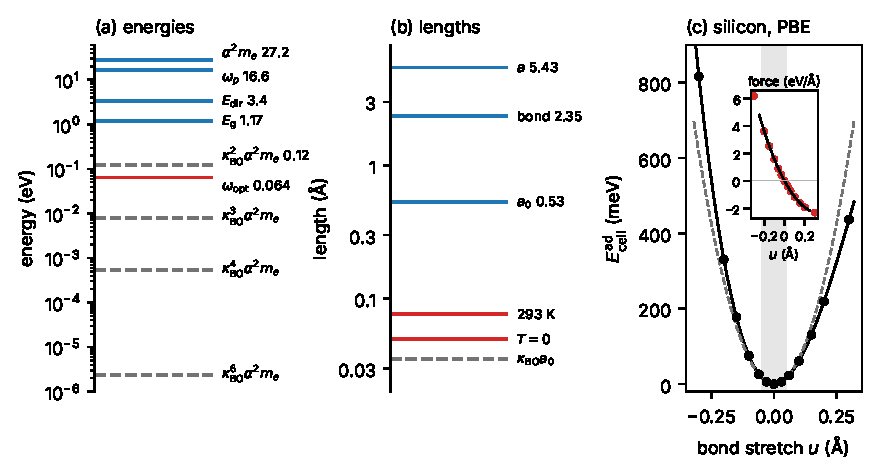
\includegraphics[width=\linewidth]{figures/ch05/fig5_1.pdf}
  \caption{Scales of electrons and nuclei in silicon. (a) Energies on a logarithmic axis, in eV. Electronic (blue): the atomic unit $\alpha^2m_e = \SI{27.2}{eV}$, the valence plasma energy $\omega_p = \SI{16.6}{eV}$, the direct gap $E_{\mathrm{dir}} = \SI{3.4}{eV}$ and the indirect gap $\Eg = \SI{1.17}{eV}$. Nuclear (red): the measured zone-center optical phonon, \SI{64.1}{meV} (\SI{15.5}{THz}), the highest vibrational energy of the crystal. Gray dashed: the Born--Oppenheimer estimates $\kappa_{\mathrm{BO}}^n\alpha^2m_e$ for $n = 2$ (phonons), 3 (cubic anharmonicity), 4 (anharmonic level shifts) and 6 (nonadiabatic level shifts), with $\kappa_{\mathrm{BO}} = (m_e/M)^{1/4} = 0.0665$ for $^{28}$Si. (b) Lengths on a logarithmic axis, in \AA: the lattice constant $a$, the bond length $\sqrt3a/4$ and the Bohr radius $a_0$ (blue). Red: the root-mean-square displacement of an atom along one Cartesian axis, $\langle u_x^2\rangle^{1/2}$, at \SI{293}{K} from a lattice-dynamical fit to neutron data and at $T = 0$ from the PBE phonon density of states. The PBE density of states uses the settings of panel (c) on a $4^3$ grid of phonon wavevectors. Gray dashed: the estimate $\kappa_{\mathrm{BO}}a_0$. (c) Energy per two-atom cell in a PBE calculation with an SG15 norm-conserving pseudopotential, a \SI{50}{Ry} cutoff, an $8^3$ grid of crystal momenta and $a = \SI{5.431}{\angstrom}$. The circles are computed at displacements in which the two atoms move in opposite directions along $[111]$ and the $[111]$ bond changes its length by $u$. The curves are a sixth-degree polynomial fit (solid) and the harmonic term $\tfrac12\Phi_{\mathrm{opt}}u^2$, $\Phi_{\mathrm{opt}} = \SI{13.6}{eV.\angstrom^{-2}}$ (dashed), from a quartic fit over $|u| \le \SI{0.1}{\angstrom}$. Shaded: $|u| < \ell_{\mathrm{zp}} = (M_\kappa\omega_{\mathrm{opt}})^{-1/2} = \SI{0.048}{\angstrom}$, the zero-point length of the coordinate $u$. Inset: Hellmann--Feynman force on $u$ (circles) and $-\dd E/\dd u$ from the sixth-degree fit (line).}
  \label{fig:5-scales}
\end{figure}

\begin{workedexample}{The small parameter of silicon}\label{we:5-kappa}
For natural silicon, $M = \SI{26.16}{GeV}$ and $m_e/M = 1.953\times10^{-5}$, so that
\begin{equation*}
  \kappa_{\mathrm{BO}} = 0.0665 , \qquad \kappa_{\mathrm{BO}}^2 = 4.42\times10^{-3} , \qquad \kappa_{\mathrm{BO}}^3 = 2.94\times10^{-4} .
\end{equation*}
The estimates \cref{eq:5.1-scales} are $\kappa_{\mathrm{BO}}a_0 = \SI{0.0352}{\angstrom}$ for the zero-point amplitude and $\kappa_{\mathrm{BO}}^2\alpha^2m_e = \SI{0.120}{eV}$ for a phonon. We compare them with the crystal (\cref{fig:5-scales}).

\emph{Energies.} The highest phonon of silicon, the optical mode at \SI{64.1}{meV}, is $\omega_{\mathrm{opt}}/\alpha^2m_e = 2.36\times10^{-3} = 0.53\,\kappa_{\mathrm{BO}}^2$: the counting, measured on the atomic scale for which it was built, is right to a factor of two. Against the gap the counting does much worse. The ratio is $\omega_{\mathrm{opt}}/\Eg = 0.0548 = 12.4\,\kappa_{\mathrm{BO}}^2$, because the gap of silicon is 23 times smaller than $\alpha^2m_e$. By \cref{eq:5.1-mixing}, $\omega_{\mathrm{ph}}/\Eg$ is the ratio that controls the mixing of excited electronic states into the ground state, so the adiabatic approximation in silicon is an order of magnitude less safe than the mass ratio alone suggests. It is still safe: the gap is eighteen phonon energies away. A semiconductor whose gap approaches the phonon energies, however, or a metal, is a different matter (\cref{sec:6.3}).

\emph{Lengths.} The zero-point amplitude of one Cartesian component is $\langle u_x^2\rangle^{1/2} = \SI{0.050}{\angstrom}$ in the PBE calculation of \cref{fig:5-scales}, 1.4 times $\kappa_{\mathrm{BO}}a_0$. At \SI{293}{K}, where thermal phonons add to the zero-point motion, a lattice-dynamical fit to neutron data gives \SI{0.0771}{\angstrom}, from $\langle u_x^2\rangle = \SI{0.005941}{\angstrom^2}$~\cite{flensburg1999lattice}, and the PBE calculation yields \SI{0.081}{\angstrom}, \SI{5}{\percent} more. This agreement suggests a similar accuracy for the zero-point value of the PBE calculation. Measured against the lattice constant, the zero-point amplitude is $\langle u_x^2\rangle^{1/2}/a = 0.0091$, seven times smaller than $\kappa_{\mathrm{BO}}$ itself. The reason for the factor of seven is the unit of length: the counting compares the amplitude with $a_0$, and the lattice constant of silicon is $10.3\,a_0$. As a fraction of the bond length, $4.4\,a_0$, the amplitude is 0.021.

\emph{Anharmonicity.} The fit of \cref{fig:5-scales}(c) has the cubic coefficient $\Phi^{(3)}_{\mathrm{opt}} = \SI{-41.5}{eV.\angstrom^{-3}}$. At $u = \ell_{\mathrm{zp}} = \SI{0.048}{\angstrom}$ the ratio of the cubic to the harmonic term of the energy is $|\Phi^{(3)}_{\mathrm{opt}}|\ell_{\mathrm{zp}}/3\Phi_{\mathrm{opt}} = 0.049$, against the estimate $\kappa_{\mathrm{BO}} = 0.067$.

\emph{Nonadiabatic shifts.} Their relative size is $\kappa_{\mathrm{BO}}^4 = m_e/M = 2\times10^{-5}$, about \SI{1}{\micro eV} on the optical phonon. A shift of \SI{1}{\micro eV} is far below the anharmonic effects and below any resolution that matters for detection.

The powers of $\kappa_{\mathrm{BO}}$ order the effects correctly, with coefficients between one half and two when the comparison is made in atomic units. The coefficients become large when a ratio is taken to a scale of the crystal itself, such as the gap or the lattice constant, and a calculation should quote ratios to these scales of the crystal.
\end{workedexample}
